\documentclass[a4paper,12pt]{article}
\usepackage[utf8]{inputenc}
\usepackage[MeX]{polski}
\usepackage[table,xcdraw]{xcolor}
\usepackage[utf8]{inputenc}
\usepackage[T1]{fontenc}
\usepackage{graphicx}
\usepackage{color}
\usepackage{mathtools}
%%%%%%%%%%%%%%%%%%%%%%%%%%%%%%%%%%%%%%%%%%%%%%%%%%%%%%%%%%%%%STRONA TYTULOWA%%%%%%%%%%%%%%%%%%%%%%%%%%%%%%%%%%%%%%%%%%%%%%%%%%%%%%%%%%%%%%%%%%%%%%%%
\title{\Huge \textbf{Politechnika Wrocławska\\[0.3in]} 
\huge Katedra Teorii Pola, Układów elektronicznych i Optoelektronicznych \\[0.2in]
\LARGE Zespół Układów Elektronicznych
}
\date{}
\author{}

\begin{document}
\maketitle

\begin{table}[h]
  \large
  \centering
  \begin{tabular}{|ll|l|}
    \hline
    \multicolumn{1}{|l|}{Data: 7.04.2015r}                  & \multicolumn{2}{l|}{Dzień: Wtorek}                                     \\ \hline
    \multicolumn{1}{|l|}{Grupa: VII}                        & \multicolumn{2}{l|}{Godzina: 12:15-15:00}                               \\ \hline
    \multicolumn{3}{|l|}{\textit{\begin{tabular}[c]{@{}l@{}}\textbf{Temat ćwiczenia:} \\ Liniowe stabilizatory napięcia\end{tabular}}} \\ \hline
    \textbf{Dane projektowe:}                               & \multicolumn{2}{l|}{}                                                     \\
    U_0=11.00 V                                             & \multicolumn{2}{l|}{I_0=0.60}                                            \\ \hline
      \multicolumn{1}{|l|}{\textbf{l.p}}                    & \textbf{Nazwisko i imię}                 & \textbf{Oceny}               \\ \hline
      \multicolumn{1}{|l|}{1}                               & Arkadiusz Ziółkowski                     &                               \\ \hline
      \multicolumn{1}{|l|}{2}                               & Jakub Koban                              &                                \\ \hline
  \end{tabular}
\end{table}
%%%%%%%%%%%%%%%%%%%%%%%%%%%%%%%%%%%%%%%%%%%%%%%%%%%%%%%%%%%%%%%%%%%%%%%%%%%%%%%%%%%%%%%%%%%%%%%%%%%%%%%%%%%%%%%%%%%%%%%%%%%%%%%%%%%%%%%%%%%%%%%%%%%%
%%%%%%%%%%%%%%%%%%%%%%%%%%%%%%%%%%%%%%%%%%%%%%%%%%%%%%%%%%%%%%%%%%%ZADANIE PROJEKTOWE%%%%%%%%%%%%%%%%%%%%%%%%%%%%%%%%%%%%%%%%%%%%%%%%%%%%%%%%%%%%%%%
%%%%%%%%%%%%%%%%%%%%%%%%%%%%%%%%%%%%%%%%%%%%%%%%%%%%%%%%%%%%%%%%%%%%%%%%%%%%%%%%%%%%%%%%%%%%%%%%%%%%%%%%%%%%%%%%%%%%%%%%%%%%%%%%%%%%%%%%%%%%%%%%%%%%
\pagebreak
\section{Zadanie projektowe}
Zaprojektować zasilacz stabilizowany o zadanych parametrach :
\begin{enumerate}
\item U_o=11.00 V$
\item  I_0=0.60 A$
\end{enumerate}
%%%%%%%%%%%%%%%%%%%%%%%%%%%%%%%%%%%%%%%%%%%%%%%%%%%%%%%%%%%%%%%%%%%%%%%%%%%%%%%%%%%%%%%%%%%%%%%%%%%%%%%%%%%%%%%%%%%%%%%%%%%%%%%%%%%%%%%%%%%%%%%%%%%%
%%%%%%%%%%%%%%%%%%%%%%%%%%%%%%%%%%%%%%%%%%%%%%%%%%%%%%%%%%%%%%%%%%%CZĘŚĆ PROJEKTOWA%%%%%%%%%%%%%%%%%%%%%%%%%%%%%%%%%%%%%%%%%%%%%%%%%%%%%%%%%%%%%%%%%
%%%%%%%%%%%%%%%%%%%%%%%%%%%%%%%%%%%%%%%%%%%%%%%%%%%%%%%%%%%%%%%%%%%%%%%%%%%%%%%%%%%%%%%%%%%%%%%%%%%%%%%%%%%%%%%%%%%%%%%%%%%%%%%%%%%%%%%%%%%%%%%%%%%%
\section{Obliczenia projektowe}

\begin{equation}
  U_0=(1+\frac{R_5}{R_6})U_{REF} \quad \to \quad (1+\frac{3k\Omega}{1k\Omega})2.75 V = 11 V
\end{equation}

\begin{equation}
  R_5+R_6 \leq \frac{U_0}{1mA} \quad \to \quad 4k\Omega \leq 11k\Omega 
\end{equation}

\begin{equation}
I_0=\frac{U_{sc}}{R_4} \quad \to \quad \frac{0.45V}{0.68\Omega}=0.66 A      
\end{equation}
%%%%%%%%%%%%%%%%%%%%%%%%%%%%%%%%%%%%%%%%%%%%%%%%%%%%%%%%%%%%%%%%%%%%%%%%%%%%%%%%%%%%%%%%%%%%%%%%%%%%%%%%%%%%%%%%%%%%%%%%%%%%%%%%%%%%%%%%%%%%%%%%%%%%
\section {Schemat projektowy}

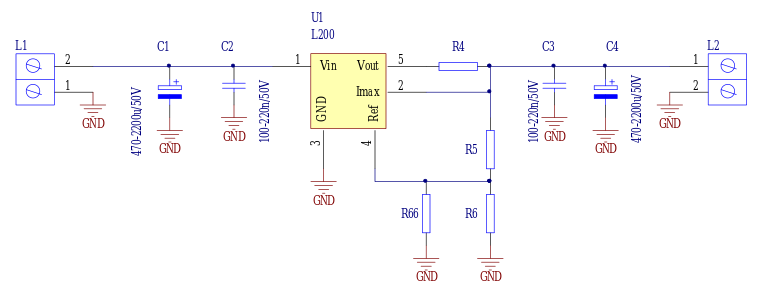
\includegraphics[scale=0.75]{schemat_ukladu}
\pagebreak
%%%%%%%%%%%%%%%%%%%%%%%%%%%%%%%%%%%%%%%%%%%%%%%%%%%%%%%%%%%%%%%%%%%%%%%%%%%%%%%%%%%%%%%%%%%%%%%%%%%%%%%%%%%%%%%%%%%%%%%%%%%%%%%%%%%%%%%%%%%%%%%%%%%%
%%%%%%%%%%%%%%%%%%%%%%%%%%%%%%%%%%%%%%%%%%%%%%%%%%%%%%%%%%%%%%%%%%%CZĘŚĆ LABORATORYJNA%%%%%%%%%%%%%%%%%%%%%%%%%%%%%%%%%%%%%%%%%%%%%%%%%%%%%%%%%%%%%%
%%%%%%%%%%%%%%%%%%%%%%%%%%%%%%%%%%%%%%%%%%%%%%%%%%%%%%%%%%%%%%%%%%%%%%%%%%%%%%%%%%%%%%%%%%%%%%%%%%%%%%%%%%%%%%%%%%%%%%%%%%%%%%%%%%%%%%%%%%%%%%%%%%%%
\section{Część laboratoryjna}
\subsection{Badanie zależności napięcia wejściowego od napięcia wyjściowego stabilizatora}
TUTAJ BRAKUJE 2 tabeli ale nie wiem czy mogę tak bezczelnie uwalić część danych :p >>DO SKONSULTOWANIA<<
\begin{table}[h]
\centering
\begin{tabular}{|r|r|}
\hline
\multicolumn{1}{|c|}{\textbf{U1{[}V{]}}} & \multicolumn{1}{c|}{\textbf{U2\_1 {[}V{]}}} \\ \hline
0                                        & 0                                           \\ \hline
2                                        & 0.2862                                      \\ \hline
5                                        & 4.0874                                      \\ \hline
5.5                                      & 4.561                                       \\ \hline
8                                        & 6.988                                       \\ \hline
8.5                                      & 7.457                                       \\ \hline
9                                        & 7.874                                       \\ \hline
10.1                                     & 8.916                                       \\ \hline
10.5                                     & 9.32                                        \\ \hline
11                                       & 9.87                                        \\ \hline
11.5                                     & 10.35                                       \\ \hline
12                                       & 10.784                                      \\ \hline
12.5                                     & 10.992                                      \\ \hline
13                                       & 10.994                                      \\ \hline
13.5                                     & 10.994                                      \\ \hline
14                                       & 10.995                                      \\ \hline
14.5                                     & 10.995                                      \\ \hline
15                                       & 10.995                                      \\ \hline
17                                       & 10.999                                      \\ \hline
19                                       & 11                                          \\ \hline
20                                       & 11.002                                      \\ \hline
25                                       & 11.007                                      \\ \hline
30                                       & 11.014                                      \\ \hline
\end{tabular}
\end{table}
\center

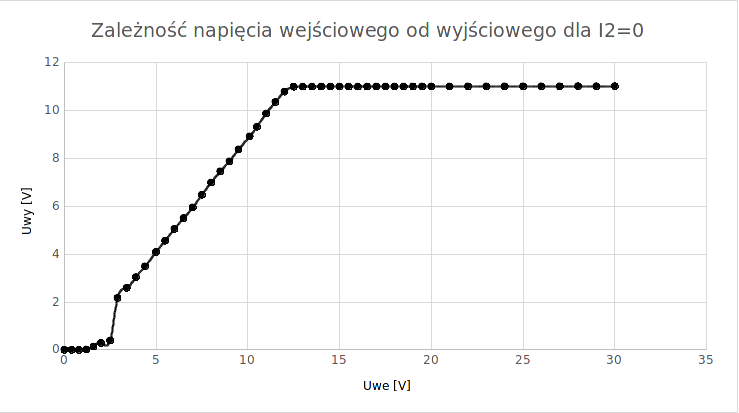
\includegraphics[scale=0.8]{Io=0}
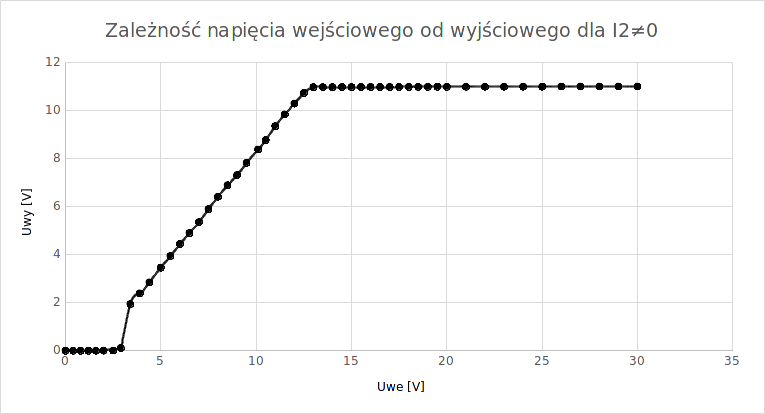
\includegraphics[scale=0.8]{ionie0}

Analizując przedstawione charakterystyki możemy zauważyć, że układ utrzymuje napięcie 11V zgodnie z założeniami projektowymi.
blablalablabalbalbalaablabablalablabalalbalaba
%%%%%%%%%%%%%%%%%%%%%%%%%%%%%%%%%%%%%%%%%%%%%%%%%%%%%%%%%%%%%%%%%%%%%%%%%%%%%%%%%%%%%%%%%%%%%%%%%%%%%%%%%%%%%%%%%%%%%%%%%%%%%%%%%%%%%%%%%%%%%%%%%%%%
\subsection{Badanie zależności prądu na wyjściu od napięcia na wyjściu dla różnych wartości rezystancji}
TU POWINNY BYC TABELKI
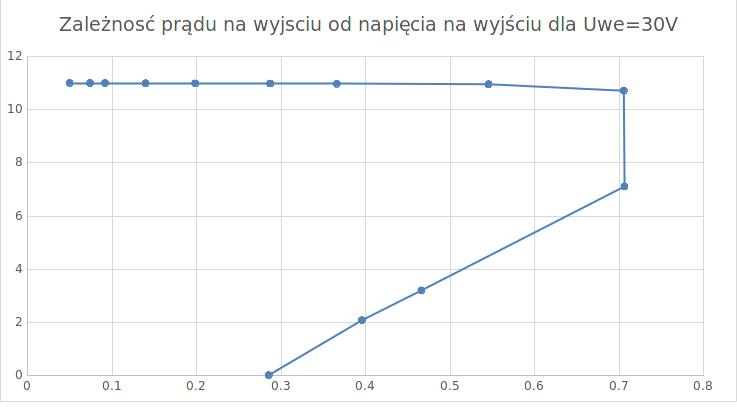
\includegraphics[scale=0.8]{u1=15}
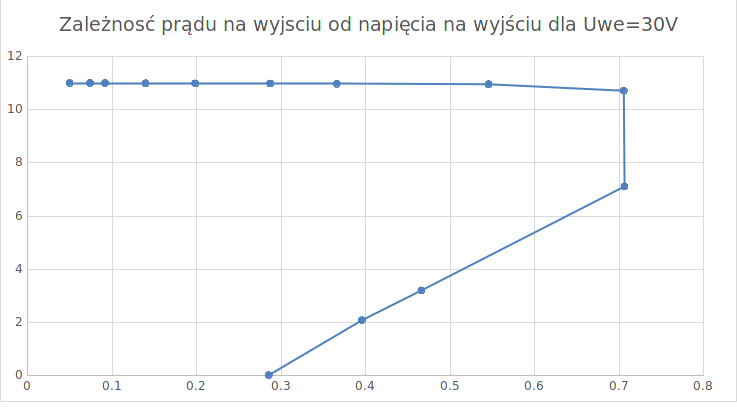
\includegraphics[scale=0.8]{u1=30}

  \section {Wnioski}
  \begin{enumerate}
  \item Zgodnie z założeniami teoretycznymi układ utrzymuje na swoim wyjściu stałe napięcie równe 11V , w związku z niedokładnością użytych elementów maksymalny prąd wyjściowy różni się od założeń jednak nie jest to duża rozbieżność (0.71 A wobec założonych 0.60 A)
  \item ad
  \item Wniosek 3
    
    \end{enumerate}
  
}

\end{document}
